\documentclass[12pt,addpoints]{exam}
\usepackage[utf8]{inputenc}
\usepackage{lastpage}
\usepackage{amsmath}
\usepackage{amsfonts}
\usepackage{amssymb}
\usepackage{enumerate}
\usepackage{mdframed}
\usepackage{array}
\usepackage{graphics}
\usepackage{graphicx}
\usepackage{listings}
\usepackage{skak}
\usepackage{tikz}
\usetikzlibrary{arrows}
\usepackage{tkz-berge}
\usepackage{algpseudocode}
\usepackage{hyperref}

% Paramètres globaux
\bonuspointpoints{point \emph{bonus}}{points \emph{boni}}
\parindent 0cm
\hqword{Question}
\hpword{On}
\hsword{Note}
\htword{Total}

% Réponses
%\printanswers

% En-tête et pieds de page
\headrule
\cfoot{\thepage /\pageref{LastPage}}
\lhead{CS Games --- Theoretical Computer Science}
\rhead{12 March 2016}
\newcommand{\headrulewidth}{0.4pt}
\newcommand{\footrulewidth}{0.4pt}

% Raccourcis
\newcommand{\bigo}{\mathcal{O}}
\newcommand{\N}{\mathbb{N}}
\newcommand{\R}{\mathbb{R}}

% Algorithmes
\algrenewcommand\algorithmicwhile{\textbf{while}}
\algrenewcommand\algorithmicfunction{\textbf{function}}
\algrenewcommand\algorithmicend{\textbf{end}}
\algrenewcommand\algorithmicdo{\textbf{do}}
\algrenewcommand\algorithmicfor{\textbf{for}}
\algrenewcommand\algorithmicif{\textbf{if}}
\algrenewcommand\algorithmicelse{\textbf{else}}
\algrenewcommand\algorithmicthen{\textbf{then}}
\algrenewcommand\algorithmicreturn{\textbf{return}}
\algrenewcommand\algorithmicrepeat{\textbf{repeat}}
\algrenewcommand\algorithmicuntil{\textbf{until}}
\newcommand{\enteteproc}[2]{\vskip\baselineskip \hspace*{\fill} \algorithmicprocedure~\Call{#1}{#2} \hspace*{\fill} \vskip\baselineskip}
\newcommand{\entetefunc}[3]{\vskip\baselineskip \hspace*{\fill} \algorithmicfunction~\Call{#1}{#2} : #3 \hspace*{\fill} \vskip\baselineskip}

% Graphes
\tikzset{VertexStyle/.style={shape=circle, fill=black, inner sep=0pt, outer sep=0pt, minimum size=1.5mm, draw}}

\begin{document}
	
\allowdisplaybreaks

\thispagestyle{empty}
~\vfill
\ifprintanswers
  \vskip 1.2cm
  \centerline{\Large\textbf{Solution de l'épreuve}}
  \vskip 0.5cm
\else
  \vskip 1.2cm
  \centerline{\Large\textbf{Theoretical Computer Science}}
  \vskip 1.2cm
\fi
\hrule \vskip \baselineskip
This challenge contains 20 questions, divided in 4 themes of 5 questions each~:
\begin{enumerate}
  \item Combinatorics;
  \item Graph Theory;
  \item Game Theory and Riddles;
  \item Probabilities.
\end{enumerate}
Each answer will be valued equally. Good luck !
\vskip \baselineskip \hrule
\vfill~
\newpage

\begin{questions}

% Combinatoire
\uplevel{The following questions are about \textbf{combinatorics}, i.e. theories concerning the counting or enumeration of objects.}

% Compter des mots
\question
A binary string $w$ avoids the pattern $u$ if it cannot be written $w = xuy$, where $x$ and $y$ are regular words (possibly empty).
\begin{parts}
  \part For any integer $n \geq 0$, let $A(n)$ the number of binary strings of length $n$ avoiding the pattern $0$. What is the value of $A(n)$ for any $n$?
  \part Similarly, let $B(n)$ the number of binary strings of length $n$ avoiding the pattern $00$. What is the value of $B(n)$ for any $n$?
  \part Similarly, let $C(n)$ the number of binary strings of length $n$ avoiding the pattern $000$. What is the value of $C(n)$ for any $n$?
\end{parts}

% Arbres binaires
\question
A \emph{binary tree} is a tree-like structure in which any vertex has at most $2$ children. For any integer $n \geq 0$, let $A(n)$ then number of trees with $n$ vertexes.
\begin{parts}
  \part Prove that the first values of $A(n)$ are what is shown in the table below~:
  \begin{center} \begin{tabular}{c|ccccc}
    $n$    & 0 & 1 & 2 & 3 & 4 \\
    \hline
    $A(n)$ & 1 & 1 & 2 & 5 & 14 \\
  \end{tabular} \end{center}
  \part It is a well-known fact that $A(n)$ validates the following equations~:
  \begin{eqnarray*}
    A(0) & = & 1, \\
    A(n) & = & \sum_{i=0}^{n-1} A(i)A(n-i-1).
  \end{eqnarray*}
  Prove these two equations. \emph{Hint~:} Think about how binary trees are recursively defined.
\end{parts}

% Numéros de téléphone
\question
How many 10-digit telephone numbers containing at least once each odd number are there (supposing all $10^{10}$ possibilities are valid)? For instance, the number $418$-$937$-$5351$ contains the digits $1$, $3$, $5$, $7$ and $9$, and thus should be taken into account.
\begin{solution}
Il est plus facile de compter d'abord le nombre $n$ de numéros de téléphones pour lesquels il manque au moins un chiffre impair. Dénotons par $N_i$ l'ensemble des numéros de téléphone dans lesquels le chiffre $i$ n'apparaît pas. Alors clairement, 
$$n = \left| N_1 \cup N_3 \cup N_5 \cup N_7 \cup N_9 \right|.$$
Évidemment, les ensembles $N_1$, $N_3$, $N_5$, $N_7$ et $N_9$ ne sont pas disjoints et donc on doit utiliser le principe d'inclusion-exclusion. Tout d'abord, notons que $|N_i| = 9^{10}$ pour $i = 1,3,5,7,9$ puisqu'il suffit d'exclure, à chaque position, le chiffre interdit (on a donc $9$ choix à chaque position). En suivant cette logique, on remarque que $|N_i \cap N_j| = 8^{10}$ pour $i,j$ impairs et distincts, puis $|N_i \cap N_j \cap N_k| = 7^{10}$, $|N_i \cap N_j \cap N_k \cap N_\ell| = 6^{10}$ et finalement $|N_i \cap N_j \cap N_k \cap N_\ell \cap N_m| = 5^{10}$.

Il ne nous reste qu'à utiliser le principe d'inclusion-exclusion. On obtient
\begin{eqnarray*}
  n & = & \left| N_1 \cup N_3 \cup N_5 \cup N_7 \cup N_9 \right| \\
    & = & (|N_1| + |N_2| + |N_3| + |N_4| + |N_5|) \\
    &   & - (|N_1 \cap N_2| + |N_1 \cap N_3| + |N_1 \cap N_4| + \ldots + |N_4 \cap N_5|) \\
    &   & + (|N_1 \cap N_2 \cap N_3| + |N_1 \cap N_2 \cap N_4| + \ldots + |N_3 \cap N_4 \cap N_5|) \\
    &   & - (|N_1 \cap N_2 \cap N_3 \cap N_4| + |N_1 \cap N_2 \cap N_3 \cap N_5| + \ldots + |N_2 \cap N_3 \cap N_4 \cap N_5|) \\
    &   & + |N_1 \cap N_2 \cap N_3 \cap N_4 \cap N_5| \\
    & = & C(5,1) \cdot 9^{10} - C(5,2) \cdot 8^{10} + C(5,3) \cdot 7^{10} - C(5,4) \cdot 6^{10} + C(5,5) \cdot 5^{10} \\
    & = & 9228691000.
\end{eqnarray*}
Le nombre de numéros de téléphone cherché est donc
$$10^{10} - 9228691000 = 771309000.$$
\end{solution}

% Chemins dans une grille
\question
Consider a grid of $r$ rows and $c$ columns (see Figure~\ref{F:grille}). In this question, we're interested in counting the paths between coordinates $(0,0)$ to coordinates $(c,r)$ by using only right (identified by the letter $r$) and up (identified by $u$) movements. Give us a formula counting the number of different paths from $(0,0)$ to $(c,r)$ for any $r,c \geq 1$.

% Nombres répétitifs
\question
An integer is \emph{repetitive} if all its digits in base $10$ are identical. For instance $33$ and $999$ are repetitive. Therefore, let $E$ a set of $12$ values from $1$ to $99$, inclusively. Prove that there are two integers $x,y \in E$ such as $x - y$ is repetitive.
\begin{solution}
Soit $X$ l'ensemble des nombres entre $1$ et $99$. Il y a au moins deux solutions à ce p
roblème.
\textbf{Solution 1}. Remarquons que si un nombre n'a qu'un seul chiffre, il est nécessairement répétitif. Par conséquent, il suffit de montrer qu'on a nécessairement deux nombres dans $E$ qui ont une différence d'au plus $9$. Pour $i = 0,1,\ldots,11$, soit $T_i = \{x \in X \mid 9i \leq x \leq 9i+9\}$ (autrement dit, les $T_i$ sont les tiroirs). Par le principe des tiroirs, si on choisit un ensemble $E$ de $12$ nombres entre $1$ et $99$, alors il existe $x, y \in E$ tels que $x \in T_i$, pour un certain entier $i$. Comme $9i \leq x,y \leq 9i + 9$, alors $|x - y| \leq (9i + 9) - 9i = 9$, c'est-à-dire que $x - y$ ou $y - x$ est un nombre répétitif.

\textbf{Solution 2}. On constate également que si $|x - y|$ est un multiple de $11$, alo rs $|x - y|$ est un nombre répétitif. Pour $i = 0,1,\ldots,10$, soit $T_i = \{x \in X \mid x \bmod 11 = i$ (autrement dit, on place les nombres dans le tiroir correspondant à l eur reste lorsqu'on les divise par $11$). Par le principe des tiroirs, il existe $x,y \in T_i$ pour un certain entier $i$, c'est-à-dire que $x \bmod 11 = y \bmod 11$. On en conclut que $(x - y) \bmod 11 = 0$, c'est-à-dire que $x - y$ ou $y - x$ est un multiple de $11$ entre $1$ et $99$, qui est un nombre répétitif.
\end{solution}

% Graphes
\uplevel{The following questions are about \textbf{Graph Theory}.
A \emph{simple graph} is a couple $G = (V,E)$ where $V$ is its set of \emph{vertices} and $E \subseteq \mathcal{P}_2(V)$ is its set of \emph{edges}, where $\mathcal{P}_2(V)$ is the set of unique pair of elements of $V$.
For instance, the graph $G = (V,E)$ defined by the sets
$$V = \{a,b,c,d\} \quad \text{et} \quad E = \{\{a,b\}, \{a,c\}, \{b,c\}, \{c,d\}\}$$
is represented by figure \ref{F:graphe}. Note: in a simple graph, there are neither multiple edges, nor loops (from an edge to a vertex to itself).}

% Familles de graphes
\question
Several simple graph families are often used. Here are some examples (see figure~\ref{F:familles})~:
\label{graphdef}\begin{enumerate}[(i)]
  \item For any integer $n \geq 1$, the \emph{complete} graph of $n$ vertices $K_n$;
  \item For any integer $n \geq 3$, the \emph{cycle} de $n$ vertices $C_n$;
  \item For any integer $n \geq 3$, the \emph{wheel} of $n + 1$ vertices $W_n$;
  \item For any integer $n \geq 1$, the \emph{hypercube} of dimension $n$ is denoted by $H_n$;
  \item For any pair of integers $m,n \geq 1$, the \emph{complete bipartite} graph $K_{m,n}$;
\end{enumerate}
For any values $n$ and $m$ as defined in \ref{graphdef}, what is the number of edges in the following graphs~:
\begin{parts}
  \part $K_n$;
  \part $C_n$;
  \part $W_n$;
  \part $H_n$;
  \part $K_{m,n}$.
\end{parts}

% Transversaux d'arêtes
\question
Let $G = (V,E)$ a simple graph. A set of vertices $U \subseteq V$ is a \emph{vertex cover} if each vertex of $G$ has at least one of its extremities in $U$, i.e for each edge $\{u,v\} \in E$, there either exists $u \in U$ or $v \in U$.
For instance in the graph illustrated in \ref{F:graphe}, the set $\{a,c\}$ is a vertex cover. A vertex cover $U$ is \emph{minimum} for $G$ if there are no vertex cover $U'$ of smaller cardinality, i.e. such as $|U'| < |U|$.

For any well-defined integers $n$ and $m$, what is the minimal vertex cover for the following graphs~:
\begin{parts}
  \part $K_n$;
  \part $C_n$;
  \part $W_n$;
  \part $H_n$;
  \part $K_{m,n}$.
\end{parts}

% Problème HAMD
\question
A graph $G$ is \emph{hamiltonian} if it possesses at least one cycle through each of its vertices \textbf{exactly} once.

Let HAMD the problem of \emph{deciding} whether a simple graph $G$ is hamiltonian or not, and let HAM the problem of \emph{finding} a hamiltonian cycle in a graph $G$ (the value \emph{nothing} is returned if no such cycle could be found). Let us consider the following functions~:
\begin{itemize}
  \item \Call{IsHamiltonian}{$G$ : graph} : boolean;
  \item \Call{HamiltonianCycle}{$G$ : graph} : cycle or \emph{nothing}.
\end{itemize}
Prove that the two problems are equally difficult minus a O(n) complexity difference. I.e, if $\textsc{IsHamiltonian}$ is temporaly constant, then we can implement $\textsc{HamiltonianCycle}$ such as it is of O(n) temporal complexity (and vice-versa). \emph{Note~:} You will need to write pseudo-code implementing both functions in relation to each other.
\begin{solution}
Supposons d'abord que \textsc{CycleHamiltonien} utilise un temps constant. Alors la fonction
\begin{algorithmic}[1]
  \Function{EstHamiltonien}{$G$ : graphe} : booléen
    \State \Return \Call{CycleHamiltonien}{$G$}~$\neq$~rien
  \EndFunction
\end{algorithmic}
a également une complexité constante.

Réciproquement, supposons que \textsc{EstHamiltonien} utilise un temps constant et considérons la fonction suivante~:
\begin{algorithmic}[1]
  \Function{CycleHamiltonien}{$G = (V,E)$ : graphe} : cycle ou rien
    \If{$\neg \Call{EstHamiltonien}{G}$}
      \State \Return rien
    \Else
      \While{il existe $v \in V$ tel que $\deg(v) > 2$}
        \State Soit $v$ un sommet de degré au moins $3$
        \For{$u \in G.\Call{Voisins}{v}$}
          \State Soit $H$ le graphe obtenu de $G$ en supprimant $\{u,v\}$
          \If{$\Call{EstHamiltonien}{H}$}
            \State $G \leftarrow H$
          \EndIf
        \EndFor
      \EndWhile
      \State \Return l'unique cycle de $G$
    \EndIf
  \EndFunction
\end{algorithmic}
Sa complexité est de $\bigo(m(m + n)) = \bigo(m^2)$ qui est bien polynomiale.
\end{solution}

% Coloriages
\question\label{Q:kparti}
Let $G = (V,E)$ a non-oriented graph and $k$ a positive integer, a function $c : V \rightarrow \{1,2,\ldots,k\}$ is a \emph{$k$-colouring} of $G$ if for any edge $\{u,v\} \in E$, we have $c(u) \neq c(v)$, i.e. if two adjacent vertices have a different colour. If $G$ can be coloured using $k$ colours, it is $k$-colourable.

A graph $G$ is $k$-partite if it possesses subsets $V_1, V_2, \ldots, V_k$ such as
\begin{enumerate}
  \item $V_1 \cup V_2 \cup \cdots \cup V_k = V$,
  \item $V_i \cap V_j = \emptyset$ et
  \item For any edge $\{u,v\}$, if $u \in V_i$ and $v \in V_j$, then $i = j$.
\end{enumerate}
Therefore, a set of vertices $V$ can be partitioned in $k$ slices such as the edges between two vertices in a same slice are forbidden.

Prove that any $k$-partite graph is $k$-colourable.

% P-équivalence coloriages
\question
Let $k$-COLORD the problem of \emph{deciding} whether a non-oriented graph $G$ is $k$-colourable and $k$-COLOR the problem of \emph{finding} such a $k$-colouring of $G$.
Prove that the problems $k$-COLORD and $k$-COLOR are equally difficult minus a O(n) complexity difference. \emph{Note~:} Question~\ref{Q:kparti} should be helpful with this.

% Jeux
\uplevel{The following questions are about \textbf{game theory and riddles}.}

% Jeu de Nim
\question
This question is based on the rules of the famous game of \emph{Nim}, a.k.a the \emph{game of matches}.
It is a two-player game, referred to as player A and player B, who must, one by one, remove 2, 3 or 4 matches from a heap.
Initially, we suppose there are $n$ matches where $n \geq 1$. The winner is the one removing the last matches.

A player has a \emph{winning strategy} if he can win a game, regardless of what the other player will do.

Explain on which conditions player A or player B has a winning strategy at Nim. \emph{Note~:} In Nim, when the value $n$ is fixed, one of the two players necessarily has a winning strategy.

% Échecs
\question
(From the book \emph{The Chess Mysteries of the Arabian Knights}, by R. Smullyan) Let us consider the following placement in a games of Checks.
\fenboard{8/8/8/1r1b4/B7/8/8/3k4 w - - 0 20}
\[ \showboard \]
The position of the white king is hidden. Furthermore, we do not know whose turn it is to play.

Guess what is the position of the white king, knowing that every previous movements were completely legit, and there is only one possible solution.
\begin{solution}
La solution se trouve à \href{https://www.chess.com/forum/view/fun-with-chess/where-is-the-king-retrograde-analysis}{https://www.chess.com/forum/view/fun-with-chess/where-is-the-king-retrograde-analysis}.
\end{solution}

% Jeu d'échecs à deux coups
\question
We will now take interest in a variation of the traditional chekers game, in which each player can play \emph{twice in one round}.
Knowing the whites begin and blacks play second, prove that with this variant, blacks cannot have a winning strategy.
\emph{Note~:} try with a proof by contradiction.

% Jet d'oeuf
\question
You find yourself in a $100$ floor building (numbered from $1$ to $100$) with $2$ eggs.
Each of these eggs has a special capacity in that there is a number $n$ between $1$ and $100$ (the number $n$ is the same for both eggs) such as~:
\begin{itemize}
  \item if you let it fall one floor between $1$ and $n$, it won't break;
  \item if you let it fall one floor between $n + 1$ and $100$, it will break.
\end{itemize}
Propose an optimal strategy to guess the value of $n$ which minimizes how many times you have to let an egg fall. You will have to explain thoroughly your answer.

% Tonneaux de vin
\question
You are a rich, unscrupulous man, possessing an unlimited number of slaves.
In six hours, you are organizing a banquet at which a large number of guests are invited.
However, you just learnt that amongst the $128$ barrels of wine you intent to serve, one has been poisoned.
You know the kind of poison used, and know it only shows symptoms of intoxication 4 hours following ingestion.
You decide to try the barrels on your slaves.

Propose a strategy that will allow you to dertermine exactly which barrel of wine has been poisoned, while minimizing the number of caualties amongst slaves. The lower the number, the more points you will be awarded.

% Probabilités
\uplevel{The following questions are about \textbf{probabilities}.}

% Générateur non-uniforme
\question
Consider a function $\Call{NonUniform}$ which returns the value $0$ with a probability of $0.7$ and the value $1$ with a probability of $0.3$.
Suppose this is the only function you have the ability to call to simulate any kind of randomness, the usual functions being unavailable.
Naturally, you may call $\Call{NonUniform}$ as much as you would like.
By using $\Call{NonUniform}$, give us the pseudo-code of a function $\Call{Uniform}$, which returns the value $0$ or $1$ with an equivalent probability.
\begin{solution}
\end{solution}

% Algorithmes et probabilités
\question
Admit that for a decision problem $P$, you are given two algorithms, $A$ and $B$.
You also have the following informations~:
\begin{itemize}
  \item When algorithm $A$ returns \emph{true}, you know the answer to $P$ is necessarily \emph{true}. However, if $A$ returns \emph{false}, it may be mistaken with a probability of $0.05$.
  \item When algorithm $B$ returns \emph{false}, you know the answer to $P$ is necessarily \emph{false}. However, if $A$ returns \emph{true}, it may be mistaken with a probability of $0.01$.
\end{itemize}
Is it possible to code an algorithm $C$ from algorithms $A$ and $B$ such as algorithm $C$ returns \emph{true} or \emph{false} without ever failing ? Justify your answer.

% Arbre binaire de recherche
\question
Consider a binary tree, suppose the following services are available for any tree $T$~:
\begin{itemize}
  \item $T.\Call{isEmpty}$ returns true iff $T$ is an empty tree;
  \item $T.\Call{content}$ returns the value contained in tree $T$'s root element;
  \item $T.\Call{size}$ returns the number of nodes in tree $T$;
  \item $T.\Call{left}$ returns the left subtree of $T$ (possibly empty);
  \item $T.\Call{right}$ returns the right subtree of $T$ (possibly empty).
\end{itemize}
Using only the above services, give the pseudo-code of a function
\begin{center}
\Call{RandomValue}{$T$ : binary tree}
\end{center}
which returns a random value from tree $T$ (we suppose one same value cannot be represented more than once, to simplify the problem).
Note that each value must have the \textbf{same probability} of being returned.
As such, you may suppose there exists a \Call{random}{$n$} function which returns a random integer between $0$ and $n - 1$ inclusively with a uniform probability.

% Échantillon
\question
Consider a set of $n$ distinct integers.
We wish to form a set of $i$ distinct integers ($1 \leq i \leq n$) sorted randomly between the $n$ integers available.
Let us suppose that once an integer was drawn from the first set, it cannot be pushed back.
To do this, let us use the following algorithm~:
\begin{algorithmic}[1]
  \Function{Sample}{$E$ : set of integers, $i$ : integer}
    \State $S \gets \emptyset$
    \While{$S.\Call{size}{} \neq i$}
      \State $e \gets $ a random element picked from $E$
      \If{$e \notin S$}
        \State $S.\Call{insert}{e}$
      \EndIf
    \EndWhile
    \State \Return $S$
  \EndFunction
\end{algorithmic}
\begin{parts}
  \part What is the probability of the algorithm not finishing ?
  \part Prove that the average number of loops is $\bigo(n\log n)$, where $n$ is the size of the set $E$ et $0 \leq i \leq n$.
\end{parts}

% Échantillon
\question
Consider an unsorted, array $T$ of $n$ integers. Let $x$ an integer with $k$ occurences in $T$. Clearly, $0 \leq k \leq n$.

We're interested in the number of values inspected when linearly searching the array $T$. Precisely, we are considering the following algorithm ($T$ is indexed from $0$)~:
\begin{algorithmic}[1]
  \Function{InArray}{$T$ : array, $x$ : element}
    \State Let $n$ the number of elements in $T$
    \State $i \gets 0$
    \While{$i < n$ \textbf{and} $T[i] \neq x$}
      \State $i \gets i + 1$
    \EndWhile
    \State \Return $i < n$
  \EndFunction
\end{algorithmic}
For any possible value of $k$, give a formula indicating the average number of values inspected.
You must provide an \textbf{exact} expression, i.e. not using $\bigo$ notation.
\emph{Note~:} Separately consider cases $k = 0$, $k = 1$ and $k > 1$.

\end{questions}

\begin{figure}
  \centering
  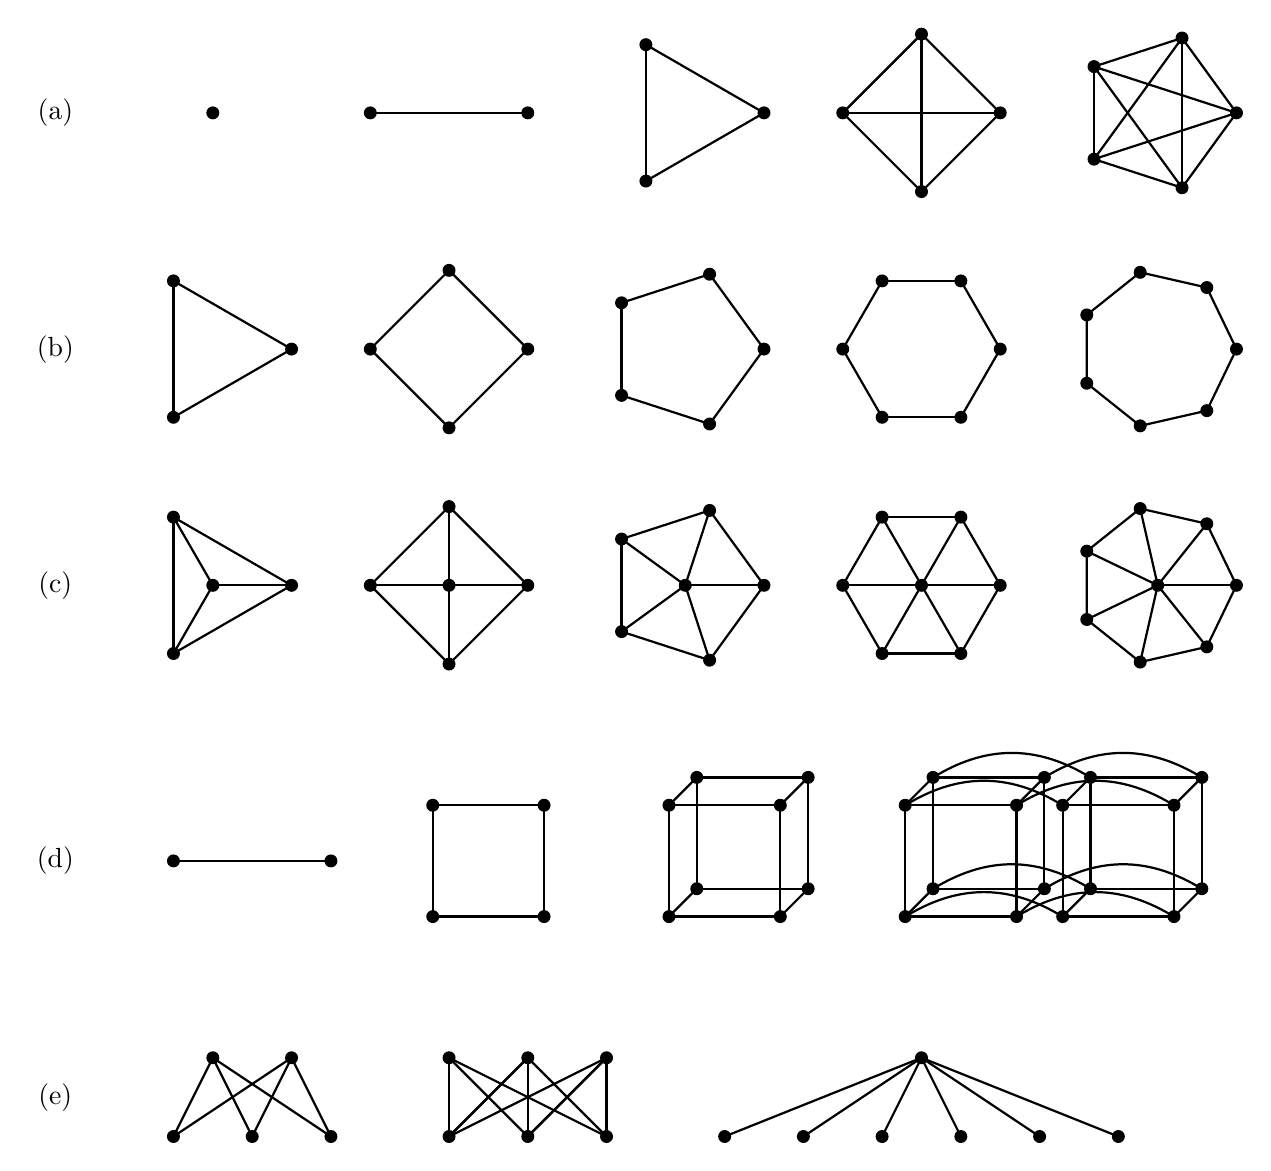
\begin{tikzpicture}
    % Complets
    \begin{scope}[xshift=-1cm, yshift=0cm]
      \node at (0,0) {(a)};
    \end{scope}
    \begin{scope}[xshift=0cm, yshift=0cm]
      \SetVertexNoLabel \Vertices{circle}{A}
    \end{scope}
    \begin{scope}[xshift=4cm, yshift=0cm]
      \SetVertexNoLabel \Vertices{circle}{A,B}
      \Edges(A,B)
    \end{scope}
    \begin{scope}[xshift=7cm, yshift=0cm]
      \SetVertexNoLabel \Vertices{circle}{A,B,C}
      \Edges(A,B,C,A)
    \end{scope}
    \begin{scope}[xshift=10cm, yshift=0cm]
      \SetVertexNoLabel \Vertices{circle}{A,B,C,D}
      \Edges(A,B,C,D,A,C,B,D)
    \end{scope}
    \begin{scope}[xshift=13cm, yshift=0cm]
      \SetVertexNoLabel \Vertices{circle}{A,B,C,D,E}
      \Edges(A,B,C,D,E,A,C,E,B,D,A)
    \end{scope}
    % Cycles
    \begin{scope}[xshift=-1cm, yshift=-3cm]
      \node at (0,0) {(b)};
    \end{scope}
    \begin{scope}[xshift=1cm, yshift=-3cm]
      \SetVertexNoLabel \Vertices{circle}{A,B,C}
      \Edges(A,B,C,A)
    \end{scope}
    \begin{scope}[xshift=4cm, yshift=-3cm]
      \SetVertexNoLabel \Vertices{circle}{A,B,C,D}
      \Edges(A,B,C,D,A)
    \end{scope}
    \begin{scope}[xshift=7cm, yshift=-3cm]
      \SetVertexNoLabel \Vertices{circle}{A,B,C,D,E}
      \Edges(A,B,C,D,E,A)
    \end{scope}
    \begin{scope}[xshift=10cm, yshift=-3cm]
      \SetVertexNoLabel \Vertices{circle}{A,B,C,D,E,F}
      \Edges(A,B,C,D,E,F,A)
    \end{scope}
    \begin{scope}[xshift=13cm, yshift=-3cm]
      \SetVertexNoLabel \Vertices{circle}{A,B,C,D,E,F,G}
      \Edges(A,B,C,D,E,F,G,A)
    \end{scope}
    % Roues
    \begin{scope}[xshift=-1cm, yshift=-6cm]
      \node at (0,0) {(c)};
    \end{scope}
    \begin{scope}[xshift=1cm, yshift=-6cm]
      \SetVertexNoLabel \Vertices{circle}{A,B,C}
      \Edges(A,B,C,A)
      \Vertex{O}
      \Edge(O)(A)
      \Edge(O)(B)
      \Edge(O)(C)
    \end{scope}
    \begin{scope}[xshift=4cm, yshift=-6cm]
      \SetVertexNoLabel \Vertices{circle}{A,B,C,D}
      \Edges(A,B,C,D,A)
      \Vertex{O}
      \Edge(O)(A)
      \Edge(O)(B)
      \Edge(O)(C)
      \Edge(O)(D)
    \end{scope}
    \begin{scope}[xshift=7cm, yshift=-6cm]
      \SetVertexNoLabel \Vertices{circle}{A,B,C,D,E}
      \Edges(A,B,C,D,E,A)
      \Vertex{O}
      \Edge(O)(A)
      \Edge(O)(B)
      \Edge(O)(C)
      \Edge(O)(D)
      \Edge(O)(E)
    \end{scope}
    \begin{scope}[xshift=10cm, yshift=-6cm]
      \SetVertexNoLabel \Vertices{circle}{A,B,C,D,E,F}
      \Edges(A,B,C,D,E,F,A)
      \Vertex{O}
      \Edge(O)(A)
      \Edge(O)(B)
      \Edge(O)(C)
      \Edge(O)(D)
      \Edge(O)(E)
      \Edge(O)(F)
    \end{scope}
    \begin{scope}[xshift=13cm, yshift=-6cm]
      \SetVertexNoLabel \Vertices{circle}{A,B,C,D,E,F,G}
      \Edges(A,B,C,D,E,F,G,A)
      \Vertex{O}
      \Edge(O)(A)
      \Edge(O)(B)
      \Edge(O)(C)
      \Edge(O)(D)
      \Edge(O)(E)
      \Edge(O)(F)
      \Edge(O)(G)
    \end{scope}
    % Hypercubes
    \begin{scope}[xshift=-1cm, yshift=-9.5cm]
      \node at (0,0) {(d)};
    \end{scope}
    \begin{scope}[xshift=1.5cm, yshift=-9.5cm]
      \SetVertexNoLabel \Vertices{circle}{A,B}
      \Edges(A,B)
    \end{scope}
    \begin{scope}[xshift=4.5cm, yshift=-9.5cm, rotate=45]
      \SetVertexNoLabel \Vertices{circle}{A,B,C,D}
      \Edges(A,B,C,D,A)
    \end{scope}
    \begin{scope}[xshift=7.5cm, yshift=-9.5cm]
      \SetVertexNoLabel
      \begin{scope}[rotate=45]
      \Vertices{circle}{A,B,C,D}
      \begin{scope}[xshift=5mm] \Vertices{circle}{E,F,G,H} \end{scope}
      \end{scope}
      \Edges(A,B,C,D,A)
      \Edges(E,F,G,H,E)
      \Edge(A)(E)
      \Edge(B)(F)
      \Edge(C)(G)
      \Edge(D)(H)
    \end{scope}
    \begin{scope}[xshift=10.5cm, yshift=-9.5cm]
      \SetVertexNoLabel
      \begin{scope}[rotate=45]
      \Vertices{circle}{A,B,C,D}
      \begin{scope}[xshift=5mm] \Vertices{circle}{E,F,G,H} \end{scope}
      \end{scope}
      \Edges(A,B,C,D,A)
      \Edges(E,F,G,H,E)
      \Edge(A)(E)
      \Edge(B)(F)
      \Edge(C)(G)
      \Edge(D)(H)
      \begin{scope}[xshift=2cm]
      \begin{scope}[rotate=45]
      \Vertices{circle}{Ap,Bp,Cp,Dp}
      \begin{scope}[xshift=5mm] \Vertices{circle}{Ep,Fp,Gp,Hp} \end{scope}
      \end{scope}
      \Edges(Ap,Bp,Cp,Dp,Ap)
      \Edges(Ep,Fp,Gp,Hp,Ep)
      \Edge(Ap)(Ep)
      \Edge(Bp)(Fp)
      \Edge(Cp)(Gp)
      \Edge(Dp)(Hp)
      \Edge[style={bend left}](A)(Ap)
      \Edge[style={bend left}](B)(Bp)
      \Edge[style={bend left}](C)(Cp)
      \Edge[style={bend left}](D)(Dp)
      \Edge[style={bend left}](E)(Ep)
      \Edge[style={bend left}](F)(Fp)
      \Edge[style={bend left}](G)(Gp)
      \Edge[style={bend left}](H)(Hp)
      \end{scope}
    \end{scope}
    % Bipartis complets
    \begin{scope}[xshift=-1cm, yshift=-12cm]
      \node at (0,-0.5) {(e)};
    \end{scope}
    \begin{scope}[xshift=1cm, yshift=-12cm]
      \SetVertexNoLabel
      \Vertices[x=0,y=0]{line}{A,B}
      \Vertices[x=-0.5,y=-1]{line}{C,D,E}
      \Edges(A,C,B,D,A,E,B)
    \end{scope}
    \begin{scope}[xshift=4cm, yshift=-12cm]
      \SetVertexNoLabel
      \Vertices[x=0,y=0]{line}{A,B,C}
      \Vertices[x=0,y=-1]{line}{D,E,F}
      \Edges(A,D,B,E,C,F,B,D,C,E,A,F)
    \end{scope}
    \begin{scope}[xshift=7.5cm, yshift=-12cm]
      \SetVertexNoLabel
      \Vertices[x=2.5,y=0]{line}{A}
      \Vertices[x=0,y=-1]{line}{B,C,D,E,F,G}
      \Edge(A)(B)
      \Edge(A)(C)
      \Edge(A)(D)
      \Edge(A)(E)
      \Edge(A)(F)
      \Edge(A)(G)
    \end{scope}
  \end{tikzpicture}
  \caption{Somme famous families of graphs. (a) The complete graph $K_n$ for $n = 1,2,3,4,5$. (b) The cycle $C_n$ for $n = 3,4,5,6,7$. (c) The wheel $W_n$ for $n = 3,4,5,6,7$. (d) The hypercube $H_n$ for $n = 1,2,3,4$. (e) The bipartite graphs $K_{2,3}$, $K_{3,3}$ and $K_{1,6}$.}\label{F:familles}
\end{figure}

\begin{figure}
  \centering
  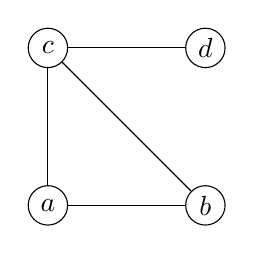
\begin{tikzpicture}[sommet/.style={draw, circle, inner sep=0pt, minimum size=5mm}]
    % Sommets
    \node[sommet] at (0,0) (a) {$a$};
    \node[sommet] at (2,0) (b) {$b$};
    \node[sommet] at (0,2) (c) {$c$};
    \node[sommet] at (2,2) (d) {$d$};
    % Arêtes
    \path (a) edge (b) edge (c);
    \path (c) edge (b) edge (d);
  \end{tikzpicture}
  \caption{The graph $G = (V,E)$, where $V = \{a,b,c,d\}$ and $E = \{\{a,b\}, \{a,c\}, \{b,c\}, \{c,d\}\}$.}\label{F:graphe}
\end{figure}

\begin{figure}
  \centering
  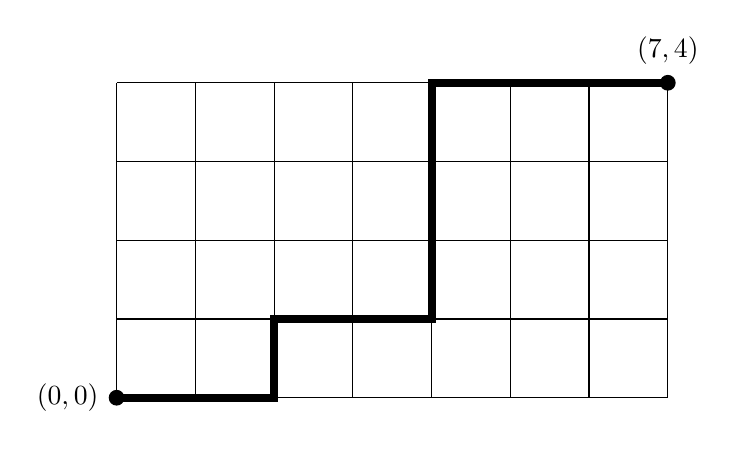
\begin{tikzpicture}[sommet/.style={fill=black, circle, inner sep=0pt, minimum size=2mm}]
    % Grille
    \draw (0,0) grid (7,4);
    % Sommets
    \node[sommet, label=180:{$(0,0)$}] at (0,0) (d) {};
    \node[sommet, label=90:{$(7,4)$}]  at (7,4) (f) {};
    % Chemin
    \draw[line width=1mm] (0,0) -- ++ (1,0) -- ++ (1,0) -- ++ (0,1) -- ++ (1,0) -- ++ (1,0) -- ++ (0,1) -- ++ (0,1) -- ++ (0,1) -- ++ (1,0) -- ++ (1,0) -- ++ (1,0);
  \end{tikzpicture}
  \caption{A grid with $r = 4$ and $c = 7$. The path $rrurruuurrr$ is drawn in bold.}\label{F:grille}
\end{figure}

\end{document}
